
%
\chapter{Assessing the utility of phase-space-localized basis functions:  exploiting direct product structure and  a new basis function selection procedure \label{ch:JCP2} }
\thispagestyle{empty}
\section{Introduction}
The manuscript in this chapter is a slight change from the previous two manuscripts of the previous two chapters as it improves on the HP doubly dense functions outlined in Chapter \ref{ch:Background}.  There is no longer an underlying set of basis functions that is being contracted using the PSL functions, but the PSL functions are being used directly.  The Hamiltonian being examined is a simplified version of the Eckart-Watson Hamiltonian instead of the general polar coordinates used in Manuscript 2.  Improvements to the matrix elements in the HP doubly dense basis, and which basis functions are chosen is also presented.

The following content of this chapter is the manuscript published as \Refc{Brown2016}.
%
\section{Abstract}
% 

In this chapter we show that it is possible to use an iterative eigensolver in conjunction with Halverson and Poirier's symmetrized Gaussian (SG)\nomenclature{SG}{symmetrized Gaussian} basis
[Thomas Halverson and Bill Poirier, The Journal of Chemical Physics,   {\bf{137}}, 224101 (2012)] 
 to compute 
accurate vibrational energy levels of molecules with as many as five atoms.
This is done,    without storing and manipulating large matrices,   by solving a regular eigenvalue problem that makes it possible to 
exploit direct-product structure.  
These ideas are combined with 
 a new procedure for selecting which basis functions to use. 
  The SG  basis we work with is orders of magnitude smaller than the basis made by using a  classical  energy criterion. We find significant convergence errors in previous calculations with SG bases.   For sum-of-product Hamiltonians, 
 SG bases large enough to compute accurate levels are 
orders of magnitude larger than even  simple pruned bases composed of products of harmonic oscillator functions.  











  



\section{Introduction}\label{2sec1}



To calculate  many accurate vibrational energy levels of a  polyatomic molecule, one must represent the corresponding  wavefunctions 
 in a basis and use  methods of numerical  linear algebra to determine the basis function  coefficients.\cite{Carter1986,Tennyson1986,Bacic1989,Bowman2008}   
  For a molecule with $D$ vibrational coordinates,  a 
wavefunction is often represented in a  direct product basis,
\begin{equation}\label{Eq.dp}
\psi({\bf{x)}} = \sum_{n_1=1}^{N_1}\sum_{n_2=1}^{N_2}...\sum_{n_D=1}^{N_D}  c_{n_1,n_2,...,n_D} ~~  ^1\theta_{n_1}(x_1)~  ^2\theta_{n_2}(x_2)...^D\theta_{n_D}(x_D) ~,
\end{equation}
%
where $^c\theta(x_c )$ is a  1D basis function for coordinate $c$,
  with maximum  indices $N_1,N_2,...,N_D$.  
The coefficients are components of eigenvectors of a matrix that represents the Hamiltonian operator in the same basis.  
A direct product basis is convenient because it enables one to  evaluate  the matrix-vector products required to use an 
iterative eigensolver to compute eigenvalues and eigenvectors of the Hamiltonian matrix at a cost that scales as $N^{D+1}$, where $N$ is a representative value of $N_c~,c=1, \cdots D$.\cite{Light2000,Manthe1990,Bramley1993,Bramley1994} 
 The   $N^{D+1}$ scaling relation is most obvious if the Hamiltonian is a sum of products (SOP) but can also be achieved for a general potential by using quadrature.\cite{Light2000} 
%
  A SOP potential energy surface
(PES) also has the advantage that it 
permits one to calculate all matrix elements from  products of 1D integrals.\cite{Jelski1996}  

%A commonly implemented sum-of-products Hamiltonian is,
%\begin{equation}\label{Eq.Hsop}
%H=\sum_{m=1}^D \omega_m\left( \dfrac{p_m^2}{2} + \dfrac{x_m^2}
%{2}\right)+\sum_{ijk}c_{ijk} x_i x_j x_k +\sum_{ijkl}c_{ijkl} x_i x_j x_k 
%x_l+...
%\end{equation}
%where $p_i=-\dfrac{\partial^2}{\partial x_i^2}$. Using a direct product of 

%



Despite the  advantages of a direct product basis, the cost of using  a direct product basis to compute     the   spectrum  of   a molecule with more than five atoms is  prohibitive.
Most important is the memory cost which scales as  $N^D$, with $D=3A-6$,  where $A$ is the number 
of atoms, for a $J=0$ calculation.  It is therefore 
advantageous to reduce the size of the basis to solve the Schr\"{o}dinger 
equation for molecules, especially when there are more than four atoms. 
\cite{Bowman2008}
There are two  established ways to reduce the basis size:  1) contract direct product bases for
sub-problems by computing eigenfunctions of reduced-dimension Hamiltonians;\cite{Bacic1989,Carter1988,Henderson1990,Wang2002,Yu2002b} 
  2) prune a direct product basis by discarding some  basis functions.\cite{Carter1986,Carter1997,Poirier2003,Dawes2005,Dawes2006}  
  Contraction can be used
with a general, i.e. not a SOP, PES.   Pruning can be used with a general PES,  if it is combined with a nondirect product quadrature or collocation.\cite{Avila2009,Lauvergnat2010,Avila2011b,Avila2015}
%
If the harmonic frequencies of all the coordinates are similar then a product harmonic oscillator basis (HOB) can be effectively pruned by retaining only basis functions
for which   $n_1+n_2+...+n_D \leq N$.    
  This reduces the basis size  from $N^D$  to
 \begin{equation}\label{Eq.HOBprune}
 \dfrac{\left(D+N+1\right)!}{D!(N+1)!} ~.
 \end{equation}
Much better, and more general, pruning conditions exist.  One can, for example, discard functions for which 
 $g_1(n_1) +g_2(n_2)+...+g_D(n_D) \le N$,  
where $g_c$ are   general functions.\cite{Avila2011b,Halverson2015}    
%
%
In this chapter,    we use a basis each of whose functions is a product of phase-space localized 
1D functions.    Conceptually, the basis we use can be thought of being obtained from 
a direct product basis by pruning, but in practice the direct product basis is never built.   
We compare the sizes of the phase-space localized (PSL)\nomenclature{PSL}{phase-space localized} with  the HOB obtained from 
 \Eq{Eq.HOBprune}.  


\section{Using PSL basis functions to compute vibrational levels}\label{2sec2}




In chemical physics, phase-space localized basis functions were first used by  Davis and 
Heller\cite{Davis1979} (DH).   They encountered significant problems and the ideas were abandoned until they were revived by Poirier et al. 
\cite{Poirier2003,Poirier2004a,Poirier2004b,Halverson2012,Halverson2015}
and 
 Tannor and co-workers.\cite{Shimshovitz2012,Shimshovitz2014}  
The use of PSL functions is motivated by the idea that a basis whose functions have   Wigner  representations
with  significant amplitude only in  and close to  the classically allowed region of phase space will be efficient.\cite{Poirier2000}  
  The hope is that it should be possible to discard PSL functions with significant amplitude (in the Wigner sense) outside the  classically allowed region.  To 
achieve good accuracy,   it will also be necessary to retain basis functions with amplitude in the tunnelling region, but the motivation is nonetheless classical.  
%
 Davis and 
Heller\cite{Davis1979}  used equally spaced Gaussians (on a phase-space grid) and found that 
they work poorly. %








%
%
The  PSL strategy we use  to obtain accurate energy levels of a Hamiltonian operator  begins with a small PSL basis and successively incorporates additional  functions into the basis
(see Section \ref{sec.expand}).   
   To understand why and how      PSL 
methods work,   it is useful, instead,  to imagine
 starting with a $direct~ product$  PSL basis large enough that  the desired energy levels are certainly  accurate and then reducing its size.   
%
Begin therefore  with a    (non-orthogonal)  direct product basis $g_n({\bf{x}})$  and     insert  an approximate resolution of the identity into the Schr\"{o}dinger equation to obtain,
\be
\sum^{f^i}_{n'}  \sum^{f^e}_{n}   \langle g_{n''} \vert   (\hat{H} - E_t)  \vert  g_{n'}  \rangle  (S^{-1})_{n',n}  \langle g_n \vert \psi_t \rangle  =0 ~,
\label{op}
\ee
where  $S_{n,n'} = \langle g_n \vert g_{n'} \rangle $.
Increase the  upper limits $f^e$  and  $f^i$ 
  until the desired energy levels are deemed sufficiently accurate,  when $f^e = f^i =F$.  
The best PSL functions are those for which 1) %  $ \sum^F_{n,n'}    \vert   g_{n'}  \rangle  (S^{-1})_{n',n}  \langle g_n \vert \approx \delta_{n,n'}$ 
$F$ is not too large    
and  %
 %
2) for the desired states,   $ \langle g_n \vert \psi_t \rangle $ is small for some $n$.
%
Accurate energies are obtained from \Eq{op},   when  elements of the  $ F \times F$ 
 ${\bf{    S^{-1}   }} $  matrix  are sufficiently close to those of an even larger  ${\bf{    S^{-1}   }} $.  
%
% 
    In a basis of Gaussians,   
 $F$ must be  huge.  The doubly dense symmetrized  Gaussian  (SG)  functions of  Halverson and Poirier\nomenclature{HP}{Halverson and Poirier} (HP) do a good job of satisfying both 1) and 2).  
%
Matrix elements of 
 ${\bf{    S^{-1}   }} $    converge more quickly as
$F$ is increased in the SG basis than in the standard Gaussian basis.
Therefore,  $F_{SG}  <  F_{Gauss}$.  See HP  for more detail.\cite{Halverson2012,Halverson2014,Lombardini2006}   
%
%  

The accuracy of the eigenvalues obtained by retaining only a subset of the $F$ PSL functions will be determined not only by the choice of the PSL functions,  but also by 
the  method  used to truncate the matrix eigenvalue problem obtained from \Eq{op}.
%
%
%
$F$ is the size of an imaginary direct product PSL basis that is certainly  large enough to compute accurate energies.   Some of the $F$ PSL functions may not be necessary and 
the eigenvalue problem  can therefore be truncated. 
%
   There are different ways to truncate.  The most obvious is to start with 
  ${\bf{ H_G W = S W E}}$,  set $f^e = f^i$,
 and then  remove rows $and$   columns of  ${\bf{ H_G  }}$ $and$   ${\bf{ S }}$.  $ (H_G)_{n,n'} = \langle g_n \vert  \hat{H} \vert     g_{n'} \rangle $.     This yields the 
  generalized    eigenvalue problem,
%
\be
 {\bf{     C^{\dagger}  H_G  C W_c} } =   {\bf{C^{\dagger}S C W_c  E^g    }}~.
\label{standard}
\ee
   ${\bf{C}}$ is a diagonal matrix with  $N_{k}$  % (the number of retained   basis functions) 
diagonal elements equal to   one  and $N_d=N-N_{k}$ (the number of discarded  basis functions) 
 elements equal to zero. 
%
As explained in \Refs{Brown2015,Brown2015b}, instead    of starting with  ${\bf{ H_G W = S W E}}$, one can start   with
 the  regular eigenvalue problem ${\bf{ H_G S^{-1} \mathcal{B} =  \mathcal{B} E}}$, where   
 $B _{n,t} = \langle g_n \vert \psi_t \rangle $.
    Rows and columns of ${\bf{ H_G S^{-1}}}$   can then be removed,  by taking $f^e  \ll  F$  , {\it without  decreasing $f^i$ },  to obtain
\be
 {\bf{     C^{\dagger}   H_G  S^{-1}   C B} } =   {\bf{   B  E^r    }}~.
\label{regulartogether}  
\ee
$ {\bf{      E^g    }}$ is  labelled by $g$ because it is  obtained from a generalized eigenvalue problem.
$ {\bf{      E^r    }}$ is  labelled by $r$ because it is  obtained from a regular  eigenvalue problem.
%
It is  also   possible to convert \Eq{standard} into a regular eigenvalue problem,  
\be
{\bf{  C^T   H_G C      \left(C^T S C\right)^{-1}       B_{pa} =  B_{pa} E^{g}}}~.  
\label{regularseparate}
\ee
%
%\ee
 $ {\bf{      E^r    }}$ is closer to $ {\bf{      E    }}$ than is $ {\bf{      E^{g}   }}$, because  it is by introducing additional approximations into 
\Eq{regulartogether}  that one obtains  \Eq{regularseparate}.   
%
The subscript $pa$ indicates that a product approximation has been made.  
Chopping matrices with   ${\bf{C}}$  would introduce no error if $both$   ${\bf{ H_G  }}$ and   ${\bf{ S }}$ were block diagonal, with
blocks being labelled by   retained and  discarded functions.  
  \cite{Brown2015b} 
 $ {\bf{      E^g   }}$ is  not as good as   $ {\bf{      E^r   }}$   because  1)  ${\bf{  C^{\dagger}   H_G  S^{-1}   C }}$ is made without discarding columns of 
${\bf{   H_G }}$ and rows of  ${\bf{    S^{-1}    }}$; 
2)    
 ${\bf{  C^{\dagger}    S^{-1}   C   \ne    ( C^{\dagger}    S    C )^{-1}   }}$ .   A   key advantage of \Eq{regulartogether}, compared to \Eq{standard}  
is that it obviates the 
need to invert $   {\bf{     C^{\dagger}    S   C} }   $. 
%
A symmetric formulation is also possible, if one starts with   ${\bf{ S^{-1/2}   H_G S^{-1/2}\mathcal{ X} = \mathcal{ X} E}}$.  
%
  Chopping the product of factors  together gives
\be
 {\bf{ C^T   S^{-1/2}     H_G S^{-1/2} C X =  X E^o}}.
\label{halftogether}
\ee
Re-arranging \Eq{standard} to make a symmetric regular eigenvalue problem gives    
%
\be
{\bf{   \left(C^T S C\right)^{-1/2}    (C^T   H_G C)   \left(C^T S C\right)^{-1/2} X_{pa}  =  X_{pa} E^{g}}}~.  
\label{halfseparate}
\ee
%
%
%
\Eq{standard},  \Eq{regularseparate}, and  \Eq{halfseparate}     have the same eigenvalues.   



More accurate energies are  obtained by  using  \Eq{regulartogether}.  Increased accuracy is almost always associated with increased cost.   Is it costly to use
\Eq{regulartogether}?     It might be costly to invert   ${\bf{       S  }}    $ and it might be costly to calculate the retained corner of   $ {\bf{  H_G   S^{-1} }} $
 because of the large number  ($F$)  of  columns of 
 $ {\bf{   H_G   }} $  and   rows of  $ {\bf{    S^{-1} }} $.    Inverting  
 ${\bf{       S  }}    $ does look  scary because the original PSL  basis is huge.     However, it is actually straightforward to obtain elements of 
 ${\bf{     S^{-1}     }}$  because the original PSL  basis is a direct product basis and therefore 
 ${\bf{     S^{-1}    =   S_1^{-1}   \otimes    S_2^{-1} \cdots    S_D^{-1}  }}$, where 
 ${\bf{    S_c^{-1}    }}$ is the inverse of a small matrix for coordinate $x_c$. \cite{Brown2015b}    
Note that, in contrast, it is  costly to invert   
 ${\bf{  C^T     S  C }}    $.     \cite{Shimshovitz2014,Shimshovitz2014b} %
%
When an iterative eigensolver is used and the PES is a SOP,  the cost of calculating the  retained corner of   $ {\bf{  H_G  S^{-1} }} $ is also not a problem, {\it{because it is never
computed}}.   Potential matrix-vector products are evaluated term by term by doing sums sequentially.   
%  
 If the PES is a SOP,
\be
 H=\sum_{\ell=1}^t  \prod_{c=1}^D \hat t^{(c,\ell)}(x_c),
\ee
and
\be
{\bf{       H_G  S^{-1}    }} =  \sum_{\ell=1}^t  [{\bf{      t^{(1,\ell)}   S_1^{-1}    \otimes       t^{(2,\ell)}  S_2^{-1}    \otimes     \cdots     \otimes  t^{(D,\ell)}  S_D^{-1}   }}] ~.
\ee


It is also possible to obviate both the inversion of     ${\bf{       S  }}    $  and the computation of   the  retained corner of   $ {\bf{  H_G  S^{-1} }} $ by using 
PSL functions      to contract a discrete variable representation (DVR) \cite{Light2000}   
%
 with $N^{DVR}$ functions.   The contraction was first proposed in 
\Refc{Shimshovitz2012}. 
Those ideas have been applied in several papers.  \cite{Shimshovitz2012,Shimshovitz2014,Machnes2016} 
  In these papers it is necessary to invert ${\bf{ G^T  G}}    $, where
  ${\bf{ G     }}$ is the 
$  N^{DVR} \times f^e$ 
DVR-PSL transformation matrix.  Instead, one can 
compute  eigenvalues of  
\be
  {\bf{   G^T H G (G^T G)^{-1}   =      G^T H (G^T)^{-1}  }}  ~.    
\label{ourst}
\ee
where 
 ${\bf{ H     }}$  is a DVR Hamiltonian matrix.  \cite{Brown2015,Brown2015b}
As long as both the DVR and the PSL basis are direct product bases,   $ {\bf{       (G^T)^{-1}  }}  $ is easily obtained by exploiting the direct product
structure.      The eigenvalue problem is,  
\be
{\bf{         G^T H (G^T)^{-1}   B_d = B_d E^d }}~.    
\ee
The  matrix of  eigenvalues, labelled by $d$ for DVR, is  equal to the eigenvalue matrix obtained from the equation of 
Shimshovitz and Tannor.\cite{Shimshovitz2012}  
%
  There is no need to introduce a 
 ``periodic von   Neumann with biorthogonal exchange'' (pvb) basis. There is no need for  periodicity. \cite{Brown2015,Brown2015b}   The resolution
 of the identity ($ {\bf{         G   (G^T G)^{-1} G^T }}$)     one inserts  to derive \Eq{ourst} is  
exact (because one is using PSL functions to contract a DVR basis).    The only approximation one makes is discarding rows and columns of the product
 $ {\bf{         G^T H (G^T)^{-1}  }}$.






In this chapter, we do not use a DVR, but instead use \Eq{regulartogether} with the SG basis of Poirier and co-workers.   Using the SG basis with 
\Eq{regulartogether}, rather than \Eq{standard}, has the  advantage that  it is somewhat more accurate.   The SG  eigenvalues we obtain from  \Eq{halftogether} are about as accurate  as those
obtained by using Poirier's Weylet basis. \cite{Poirier2003,Poirier2004a,Poirier2004b}  
   Halverson and Poirier introduced the SG basis because it is ``much more convenient''.\cite{Halverson2012}    
They use it with \Eq{standard}.  
%


A crucial part of the strategy of using PSL functions is deciding $which$ ones to put into the working basis.  It is straightforward to build a basis that includes
PSL functions whose phase space centres are in a    classically allowed region of phase space.   
   The idea that the  classical region associated with energy $E$, denoted $\mathcal{R}_E 
$  
by Poirier,  
 must be important  for computing states with energy less than $E$ motivated  the 
development of PSL basis methods.    There is no doubt that 
 PSL functions  in    $\mathcal{R}_E $   must be in the working basis.   The problem is that wavefunctions of states with energy less %
%
 than $E$ have tails that 
extend beyond      $\mathcal{R}_E $.  
     It is therefore necessary also to include PSL functions with amplitude outside  the classical region.   The  simplest  way to ensure  that such 
PSL functions are in the working basis is to  use the functions in the region 
 $\mathcal{R}_{E_{thres}}$, 
 where $  {E_{thres}} >  E$.      
 In this chapter we use a better criterion for determining which 
PSL to include in the working basis.   The ideas are related to those of \Refs{Shimshovitz2014,Brown2015b}.  




There are three favourable properties of  the approach of this chapter. 
  First, it  makes it possible to use iterative eigensolvers and thereby obviate the need to store (and compute) the Hamiltonian and overlap  matrices.  Note, however, that 
 Poirier et al. have done impressive calculations using huge parallel computers and direct eigensolvers.\cite{Halverson2012,Poirier2004b}
%
  Second,  we obtain results about as accurate as those obtained
with a Weylet basis but using  a  simpler SG basis.  Third,  we introduce a better way of choosing which product PSL functions to include in the final basis. 











\section{Advantage of truncating the product  ${\bf{ H_G S^{-1}}}$:       1D  SG results\label{Sec.chop}}

We  use the doubly dense symmetrized Gaussian basis proposed 
%
in  \Refs{Lombardini2006,Halverson2012}.  In  atomic units ($\hbar=1$) a 1D SG function is 
\begin{equation}
d_n\left(x\right)=\exp\left[-\alpha\left(x-
x_{n_x}\right)^2\right]\cos\left[p_{n_p}\left(x-x_{n_x}-\dfrac{dx}{2}\right)\right] ~,   
\end{equation} 
where $n$ is a composite index including  $n_x,n_p$.  $x_{n_x}$ and $p_{n_p}$ are the centres of 
the SG functions in phase-space with $x_{n_x}=n_x\sqrt{\pi}+\sqrt{\pi}/2$ and  
$p_{n_p}=n_p\sqrt{\pi}+\sqrt{\pi}/2$,  both $n_x,n_p$  are  integers, and $n_p\geq0$.  
This is the grid spacing used in \Refc{Halverson2012} and with $\alpha=1/2$ 
it generates  a basis that is complete but not over-complete. 


To assess the different truncated eigenproblems, we first    use this basis to compute energy levels of 
\begin{equation}\label{Eq.1dharm}
H=-\dfrac{1}{2}\dfrac{\mathrm{d}^2}{\mathrm{d}x^2}+\dfrac{1}{2}x^2 ~.   
\end{equation}
%
 The original  basis   (whose size is $F$)
is built from a    $40\times 20$ phase-space grid with $n_x=-20,-19. \cdots, 19,n_p=0,1,2, \cdots 19$.   
%
 It covers a square region of phase-space, \newline
  $x\in 
\left[-20\sqrt{\pi},20\sqrt{\pi}\right],\;p\in    
\left[-20\sqrt{\pi},20\sqrt{\pi}\right]$. 
All the matrix elements were calculated  analytically and the matrices
 $ {\bf{   H_G   }} $   and  $ {\bf{   S    }} $  were built. 
In this section,  the functions included in the working basis are those whose centres are inside the region
$\mathcal{R}_{E_{thres}} $,     
, i.e., those for which  $
\dfrac{p_{n_p}^2}{2}+\dfrac{x_{n_x}^2}{2}  < {E_{thres}}= 55$.    
There are  $56$ retained basis functions. 

%


%
In Figure  \ref{Fig.ddhalfE},    we compare \Eq{standard} and \Eq{halftogether} by plotting them together with eigenvalues of the full problem,  ${\bf{ H_G W = S W E}}$.
\Eq{standard} is used in \Refs{Halverson2012,Halverson2015,Davis1979}. 
%
 It is clear that all 56   energies computed with  the full $40\times 20$ basis  are accurate.  
The SG basis of HP is designed to  
%
%
reduce the effect  of the approximations required to 
get \Eq{halfseparate} (equivalent to   \Eq{standard})   from \Eq{halftogether}.     The similarity of the two curves in    Figure  \ref{Fig.ddhalfE} confirms the advantages of the SG basis. 
%
% 
Energies obtained from  \Eq{halftogether} are, however, always more accurate, see   Figure  \ref{Fig.ddhalfE}.
  The accuracy difference is larger for smaller energies.   The 
 ground state energy computed with   \Eq{halftogether}    has    an extra digit of precision.
%
Results obtained from \Eq{standard} and  \Eq{halftogether} are less similar when the PSL functions are  Gaussians.    
%
With SG functions, the difference between results obtained with  \Eq{standard} and \Eq{halftogether}, plotted in 
 Figure  \ref{Fig.ddhalfE}, 
 is similar to the difference between results obtained with 
Poirier's Weylet basis \cite{Poirier2003,Poirier2004a,Poirier2004b} 
and with     HP's SG basis using   \Eq{standard}. 
%
  This difference has been noted by HP.   \cite{Halverson2012}
Energies obtained from \Eq{halftogether} should be very close to those obtained with Weylets.
%


%
%
\begin{figure}[t]
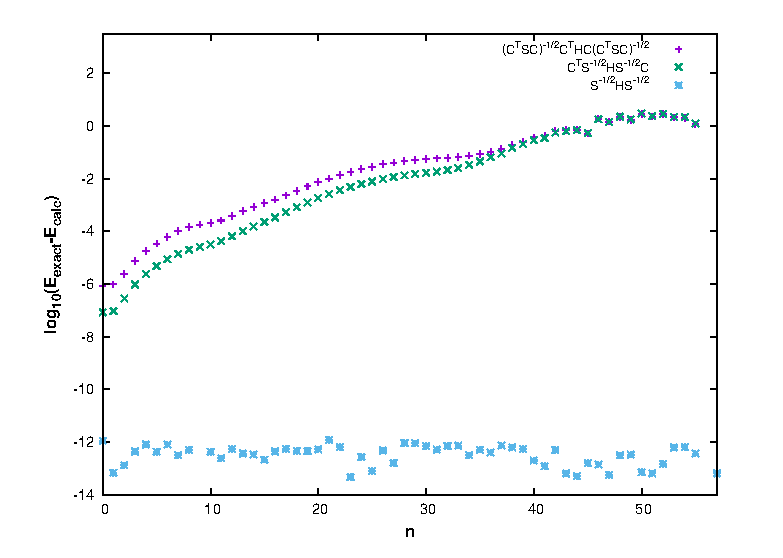
\includegraphics[width=6.5in]{./JCP2/fig1.eps}
\caption[Comparison of different symmetric chopping schemes for the harmonic oscillator]{Comparison of the accuracy of \Eq{halftogether} and \Eq{halfseparate} (or \Eq{standard}) for 
the harmonic oscillator Hamiltonian.  The starting basis of $800$ SG functions  is reduced to 
$56$ basis functions.  $n$ on the $x$ axis labels an  eigenvalue.  \label{Fig.ddhalfE}}
\end{figure}





 To use \Eq{halftogether}, which gives slightly better accuracy,   it is necessary to compute the retained corner of $ {\bf{    S^{-1/2}   H_G   S^{-1/2} }} $,
which  requires  summing over all 800 rows and  columns of    $ {\bf{  H_G   }} $.
In contrast,  to use  \Eq{standard}, one must only deal with $56 \times 56$ matrices.   For a multidimensional problem,  summing over all the SG functions in the 
original basis is not an option. However, for a multidimensional problem  $ {\bf{    S^{-1/2} }} $ can be computed and stored by exploiting its direct product
structure and if the PES is a SOP,  matrix-vector products can be evaluated without calculating the retained corner of $ {\bf{     S^{-1/2}   H_G   S^{-1/2}         }} $.   
%
Using Poirier's Weylet ideas,  it is possible to implement     \Eq{halftogether} without     summing over all the SG functions in the 
original basis. 





%
  In Figure \ref{Fig.ddoneE}   we compare \Eq{regulartogether}  and \Eq{standard}.  
  According to   \Refc{Brown2015b}, the eigenvalues of \Eq{regulartogether} should be significantly more 
  accurate than those of \Eq{standard}. 
  This is indeed the case.  
%
There are two reasons.   
First, in  \Eq{regulartogether}  800 columns of    ${\bf{     H_G     }} $ and 800 rows of  ${\bf{   S^{-1}          }} $  are retained.   
Second,   ${\bf{   (C^T S C)^{-1}          }} $ $ \ne {\bf{  C^T  ( S )^{-1}       C   }} $.
%
%




%JB added back X discussion
 The eigenvalues of \Eq{regulartogether}  are more accurate than those of  \Eq{halftogether} due to the fact that 
${\bf{    B   }} $ with elements  
 $B _{n,t} = \langle g_n \vert \psi_t \rangle $  has columns with small components and   the 
 corresponding elements of 
  ${\bf{   X = S^{-1/2}  B   }} $  are not as small.  They are not as small  because   the small components of   ${\bf{    B   }} $   get smeared out
 by  ${\bf{  S^{-1/2}       }} $.   This means that 
less error is introduced by chopping    ${\bf{     H_G  S^{-1}    }} $. 
We shall therefore use  \Eq{regulartogether}  for multidimensional calculations.   For multidimensional problems 
 $ {\bf{    S^{-1} }} $ will be  computed and stored by exploiting  direct product
structure.  For SOP PESs,  we  shall take advantage of direct product structure and not calculate  the  retained corner of $ {\bf{       H_G   S^{-1}         }} $.   



%
%
\begin{figure}[t]
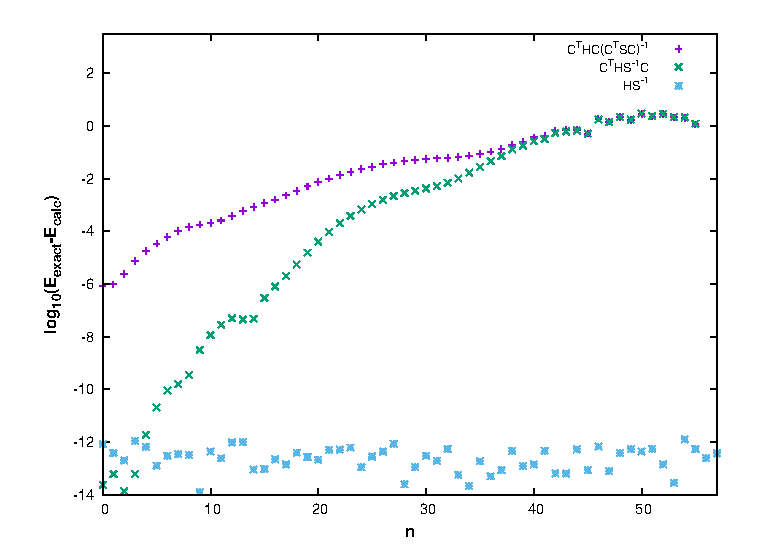
\includegraphics[width=6.5in]{./JCP2/fig2.eps}
\caption[Comparison of different asymmetric chopping schemes for the harmonic oscillator]{Comparison of  the accuracy of \Eq{regulartogether} and \Eq{regularseparate} (or \Eq{standard})  for the 
harmonic oscillator Hamiltonian.   A  starting basis with  $800$ SG functions is reduced to $56$ 
basis functions. $n$ on the $x$ axis labels an eigenvalue.    \label{Fig.ddoneE}}
\end{figure}





%

\section{Expanding a  basis of PSL functions\label{sec.expand}}

%


One wishes to choose a working basis 
that includes only the PSL functions corresponding to  large components of  the     columns of ${\bf{    B  }} $  associated with  desired energies.
It is not possible to solve the Schr\"{o}dinger equation in the full basis (with   $F $ functions).  Instead, one needs some 
means of determining which are the important functions.  
%
%
%  
%
 For the Hamiltonian,     

\begin{equation}
H=-\dfrac{1}{2}\dfrac{\mathrm{d}^2}{\mathrm{d}x^2}+\dfrac{1}{2}x^2+\dfrac{1}
{10}x^3+\dfrac{1}{100}x^4~,
\end{equation} 
% 
%
putting SG basis functions into  $\mathcal{R}_{E_{thres}} $  works less well.  



% 
%
Clearly,  it would be better to determine which PSL functions to include in the  working basis  by using  elements of   ${\bf{    B  }} $.    There are several schemes for expanding 
a PSL basis so that it includes the important functions.  \cite{Shimshovitz2014,Brown2015b}
%
\begin{figure}[t]
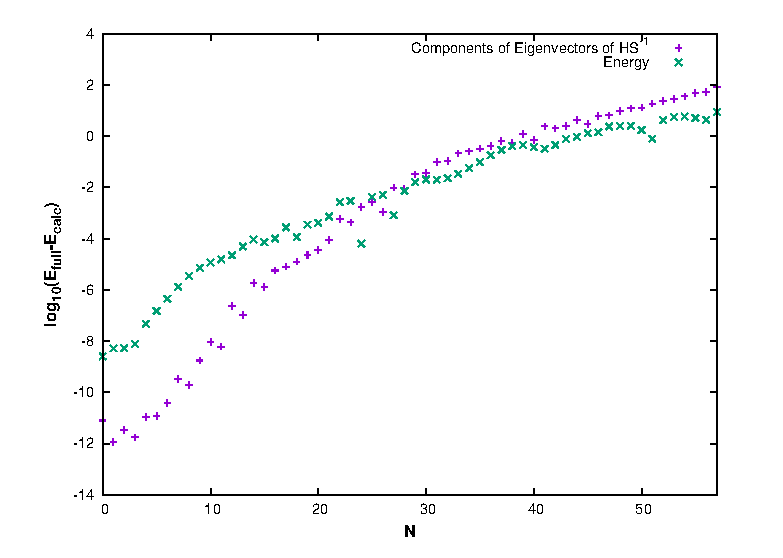
\includegraphics[width=6.5in]{./JCP2/fig3.eps}
\caption[Comparison of accuracy of classical energy and basis building scheme using phase-space localized basis functions.]{Comparison of the accuracy achieved by using a basis  composed of the 56 functions whose classical energy  is less than a threshold of 55,
%
and a basis 
composed of  the 56 functions for which components of eigenvectors of ${\bf{  H S^{-1}}}$  are largest        
 The latter basis is clearly better.\label{Fig.coefvE}}
\end{figure}
%
The scheme we use in this chapter begins by identifying 
a small set of  
 basis functions that are
 important and then adding new functions that are in some sense close 
to those deemed important.  
%
If  $\vert B_{nm}\vert$ is tiny then removing the $n$th basis function will have almost no effect on the    $m$th eigenvalue.   \cite{Brown2015b}  
It is also true that  if   $\vert B_{nm}\vert$  is large the  $n$th basis function is  important for calculating the    $m$th eigenvalue. 
We, therefore, deem a basis function important if 
$c^{sum}_n=\sum_{m=1}^{10} \left|  B_{nm}  \right|$ is large.     $c^{sum}_n$ is  the sum of the      
absolute values of  the components  of 
the 10 eigenvectors whose eigenvalues are smallest,   for a given basis function $n$. 
  %
%
If we retain the 56 basis functions with the largest values of $c^{sum}_n$,  we obtain a 
%
working basis 
with which the first 25 eigenvalues are 
 more accurate than those computed using  the 56 
functions that satisfy the $\mathcal{R}_{E_{thres}} $ criterion,  
  see Figure \ref{Fig.coefvE}. 
This establishes the advantage of using eigenvector components to determine which functions are 
included in the working basis  
%
to calculate the lowest energy eigenvalues.
For typical  spectroscopic problems, it is most important to calculate the lowest eigenvalues accurately.  However, if one wishes  to calculate a large number of eigenvalues 
to a fairly low accuracy level, a basis made with  the $\mathcal{R}_{E_{thres}}$ criterion might be better.  



  





%
%
For a real multi-dimensional problem, we want to build the working basis without knowing  ${\bf{   B}}$ and we therefore iteratively expand the basis  by 
successively adding to the  basis new functions, $d_{{\bf{n'}}}$,   
 whose phase-space centres are close to those of functions  $d_{{\bf{n}}}$  already in the basis and for which 
 $c^{sum}_{\bf{n}}$  is large.
For a multi-dimensional problem $  {\bf{n}} $ = $\{ n_1,n_2,   \cdots, n_D \} $.     
The  strategy is based on the  assumption  that  both wavefunctions and the basis functions  are  localized  and smooth
in phase space. 
%
%
To make the basis,  we first create a starting basis and then add functions to it.   Functions in the starting basis are those whose 
 phase-space centres are in a region      
 $\mathcal{R}_{E_{thres}} $  for a Hamiltonian that is the separable harmonic part of the full Hamiltonian and with a small $E_{thres}$.
%
The classical energy that corresponds to a PSL function is a sum of positive terms, one for each of the $2D$ 
terms in the   separable harmonic Hamiltonian.
To build the starting basis one must, in  principle, 
 consider for possible inclusion  all phase-space points in a huge direct product grid and for each of these points add up contributions 
from each of the $2D$ terms to obtain an energy, $E_{sum}$, and reject those functions for which   $E_{sum}  >  E_{thres} $.
%
 In practice,  for a given point, there is  no need to add 
contributions for all $2D$ terms because 
 when   $E_{sum}  >  E_{thres} $ there is no need to add contributions (all positive)  from other terms.   
%
There is also no need to loop over all points on the huge direct product grid.  
Assume the top loops are  over $n_{x_1}$ and $n_{p_1}$ and the bottom loops are over
 $n_{x_D}$ and $n_{p_D}$.  If, when considering for possible inclusion, 
  the         phase-space point $ n_{x_1},n_{p_1},   n_{x_2},n_{p_2},   \cdots   n_{x_D},n_{p_D} $,%
 after summing over terms  for $c=1,2,3$ ~  ,  
    $E_{sum} >  E_{thres} $,       
then there is no need to execute the remaining loops, for  $c=4,5, \cdots,  D$.
%
%
If nothing were 
 done to avoid looping over all the points of  the   huge direct product basis and all  the $2D$ terms,  the cost of determining which PSL to include in the starting basis would 
scale  exponentially with    $D$.     
 Halverson and Poirier\cite{Halverson2015} use    a more    
sophisticated method,  that defeats this exponential scaling,
to define their final basis which is defined so that it contains   all PSL functions with centres in 
 $\mathcal{R}_{E_{thres}} $,  for the full  Hamiltonian.  Determining only a starting basis is simpler.   







To generate the basis we do a set of Arnoldi calculations with increasing basis sizes.  The first Arnoldi calculation is done with the starting basis of the 
previous paragraph.      $c_{{\bf{n}}}^{sum}$ values are  calculated for each of  the $N_k$ functions in the starting basis.
  The   $c_{{\bf{n}}}^{sum}$     are then sorted using the Quicksort algorithm. \cite{Hoare1961}  
%
 We  add  to the basis neighbours of 
the PSL function with the largest  $c_{{\bf{n}}}^{sum}$, then neighbours of the PSL function with the 2nd largest  $c_{{\bf{n}}}^{sum}$, etc.  
When the size of the basis has been increased 5\% we stop adding functions.   
For a given ${\bf{n}}$, corresponding to   the phase space point $(n_{x_c}, n_{p_c})$, $c=1,2,...,D$, %
 the neighbours added  are  PSL functions  
with phase space points  $(n_{x_c}, n_{p_c})$, which are 
 1)    $n_{x_c}' = n_{x_c}$   and   $ n_{p_c}'$     
=  $n_{p_c}'+1$;
 2)    $n_{x_c}' = n_{x_c}-1$  and  $ n_{p_c}'$  =  $1$ ;
 3)   $n_{x_c}' = n_{x_c} +1$   and  $ n_{p_c}$  =  $1$.  
There are a total of $3 D$   neighbours.  
%
The basis composed of the starting basis and the    neighbours is the first expanded basis.  It  in turn is expanded to form the second expanded basis 
by doing another Arnoldi calculation and adding more neighbours.   The   process is repeated until we deem energy levels converged.   Each new basis is  
 5\% larger than the previous basis. 
%
We maintain a list of functions in the basis with index $m$,  and a list of $c_{{\bf{n}}}^{sum}$ values for functions in the basis for which we have not yet checked whether their neighbours should be included.  
%
   The $m$ corresponding to the largest $c_{{\bf{n}}}^{sum}$ values can be obtained from ${{\bf{n}}}$ using the mapping in the next section.      
  Before adding a neighbour, we use the same  mapping  to determine whether   it is  already in the basis.   
 %
The initial list  of $c_{{\bf{n}}}^{sum}$ values 
 includes   
all the  functions in the starting basis.     
% 
%
%
%
After adding     neighbours   for a particular basis function $\bs{n}$   to a  basis, 
we remove that     $c_{{\bf{n}}}^{sum}$   %
 from the list of  $c_{{\bf{n}}}^{sum}$   for    not-yet-checked functions. 
 $c_{{\bf{n}}}^{sum}$ is calculated only for functions in the not-yet-checked list.
%%
 This saves  computation time  in later  iterations due to the fact that many   PSL functions  have already had  their  phase-space neighbours added to the  basis. 
%  
%
%
It is perilous to determine  whether an eigenvalue is converged by comparing values at different basis sizes because the plot of an eigenvalue as a function of basis size 
may have plateaus.  
One way to ensure that eigenvalues are converged is to add basis functions until    the  $c_{\bs{n}}^{sum}$  of all the basis functions are all less than a small cutoff value.
  When  all $c_{\bs{n}}^{sum}$ in the not-yet-checked  list are below the  cutoff 
value, convergence is    achieved.
%
It might also be possible to use residuals to monitor convergence.  








\section{Computing a spectrum\label{sec.compit}}



Using the ideas of the previous sections, it is possible to sculpt a basis for a Hamiltonian.   Unfortunately, even the basis that includes only
the most important functions from a huge direct product basis is itself so large that most computers do not have enough memory to calculate eigenvalues of the 
basis representation of the Hamiltonian using methods of direct linear algebra.
Phase-space basis methods that require inverting an overlap matrix for the retained PSL functions are similarly limited by the need to store and manipulate large matrices.  \cite{Shimshovitz2014,Machnes2016} 
   One option is to use massively parallel computers.   \cite{Halverson2012,Halverson2014}    Another is 
to use an  iterative eigensolver.    
  Iterative eigensolvers  have been used to compute vibrational spectra for many years. \cite{Light2000,Bowman2008,Huang1999,Roy1995,Bramley1993,Mandelshtam1997,Iung1989,Yu1997,Chen1998} 
%
   They have the obvious advantage that they obviate the need
to store the Hamiltonian matrix.   Nevertheless, they are only efficient if there is a good way of evaluating matrix-vector products.    When the basis is a direct product,
 matrix-vector products can be efficiently evaluated by doing sums sequentially.\cite{Light2000,Bramley1993}   
%
  To use this idea, there is no need to build a Hamiltonian matrix because 
matrices representing 1D factors are sequentially  applied        to vectors.   These ideas cannot be used when the basis does not have product structure and a pruned basis 
built as explained in the previous section does not have product structure.    Avila and Carrington have shown that, despite pruning, it is possible to efficiently 
evaluate matrix-vector products by doing sums sequentially, {\it{ if basis functions are retained by imposing a pruning condition that itself has structure}}.\cite{Avila2009,Avila2011,Avila2015}
%
 A basis 
chosen to include only the important PSL functions will, in general, not have exploitable structure.    New ideas  are therefore required to evaluate matrix-vector products, in order to make iterative eigensolvers useful.


The technique we use to evaluate matrix-vector products only works if the Hamiltonian is a SOP.   Matrix-vector products are evaluated term by term and, for each term, factor by factor.  
We compute eigenvalues of $\bs{ H_G S}^{-1} $  where  $\bs{ H_G = \sum^t_{\ell} H_{\ell}  } $ and
${\bf{ S  = S_1 \otimes S_2 \otimes \cdots  S_D }}$.     To explain the ideas we shall focus on a single term,
  \be
{\bf{  H_{\ell}   = H^{\ell}_1 \otimes H^{\ell}_2 \otimes \cdots  H^{\ell}_D }} ~,  
\ee
 and therefore on    $\bs{ H_{\ell}}\bs{  S^{-1}}  =  \bs{H^{\ell}_1}\bs{ S_1^{-1}}  \otimes \bs{H^{\ell}_2  S_2^{-1}}   \otimes \cdots  \otimes  \bs{H^{\ell}_D S_D^{-1}}  = \bs{^1O^{\ell}}    \otimes  \bs{^2O^{\ell} }   \otimes    \cdots  \otimes \bs{ ^DO^{\ell} }   $.   
Note that many of the  
   ${\bf{  H^{\ell}_c}}, c=1,2, \cdots D$ factors may be (1D) overlap matrices.    
 If the PES is a Taylor Series then other  ${\bf{  H^{\ell}_c}}$   are  $\bs{x_c}^i, i=1,2,3,4$; others are  $\bs{  p_c}^2$
   We shall drop the superscript ${\ell}$ in the rest of this section.    
%
For one factor of one term,  the matrix-vector product one must evaluate could be written 
%
% 
\begin{equation}  
v_{n_{x_1}',n_{p_1}',...,n_{x_c}',n_{p_c}',..,n_{p_{D}}'}
= \sum_{n_{p_{c}}=1}^{N_{p_c}}
  \sum_{n_{x_c}=1}^{N_{x_c}}
%
      \bs{ ^cO}_{n_c^{\prime},n_c}
z_{n_{x_1}',n_{p_1}',...,n_{p_{c-1}}',n_{x_c},n_{p_c},n_{x_{c+1}}',n_{p_{c+1}}',..,n_{p_{D}}'} ~,
%
\label{jason-type}
\end{equation}
where $n_{x_c}$  and  $n_{p_c}$ are  position and momentum labels for coordinate $x_c$,  and   $n_c$  is a composite label that includes  
 $n_{x_c}$  and  $n_{p_{c}}$.   $ \bs{ ^cO}_{n_c^{\prime},n_c}$ depends on  $n_{x_c}$  and  $n_{p_{c}}$  and  $n'_{x_c}$  and  $n'_{p_{c}}$   because each 1D basis function has  both 
 position and momentum labels.   
%
  The vectors are stored in a 1D array indexed by $m$ and the matrix-vector product      is
  \begin{equation}
  \begin{split}  
v(m'(n_{x_1}',n_{p_1}',...&,n_{x_c}',n_{p_c}',..,n_{p_{D}}'))
= \\ &\sum_{np_{c}=1}^{Np}
  \sum_{nx_c=1}^{Nx}
%
      \bs{ ^cO}_{n_c^{\prime},n_c}
z(m(n_{x_1}',n_{p_1}',.. ,n_{p_{c-1}}'  ,n_{x_c},n_{p_c},  n_{x_{c+1}}',..,n_{p_{D}}')) ~,
%
\end{split}
\label{eq.sopmv}
\end{equation}
The sums must be done for  $m'$ =$ 1, 2, \cdots,  N_k$.
 Knowing a value of $m'$ one finds values of ${n_{x_1}',n_{p_1}',...,,n_{x_c}',n_{p_c}',...,n_{p_{D}}'}
$ from a $N_k \times 2D$ table that is stored.   The table is denoted $A$.  Its 
$m'$th row contains   the $2D$ ${n_{x_1}',n_{p_1}',...,n_{x_c}',n_{p_c}',...,n_{p_{D}}'}
$   labels  for the  $m'$th      basis function. 
%
Note that we are not, as is often the case when 
evaluating matrix-vector products in a pruned basis, 
transforming the input vector into the output vector, index by index sequentially, with  $D+1$  nested loops.
%
   When indices are transformed sequentially, the 
transformed and untransformed indices are separately constrained.  In this case, the length of intermediate vectors increases and then 
decreases.   \cite{Avila2009,Wang2001c}    
% 
Instead, for each factor, the vector on the LHS of \Eq{eq.sopmv} has only as many elements as there are retained basis functions.  
This is similar to the strategy of \Refc{Cooper2009}.
%JB should this go above? "Note that we are not..."
 





It remains to explain how knowing  $
{n_{x_1}',n_{p_1}',...,  n_{x_{c-1}}',n_{p_{c-1}}',n_{x_c},n_{p_c},n_{x_{c+1}}',n_{p_{c+1}}'...,n_{p_{D}}'}$ one finds $m$, which labels the input vector.    In principle this could be done 
by storing a 
 $D$ 
dimensional array  with  $(N_xN_p)^{D}$ elements,  whose value is  $m$, if the corresponding function is in the basis, 
and  0, if the corresponding function is not in the basis.   
Of course, this is impossible because the array is huge.  It is also not necessary because many of the elements of the array would be zero.   
Instead, we use a recursive mapping.   It is determined by making a list of retained 
 $
{n_{x_1},n_{p_1},...,,n_{x_c},n_{p_c},...,n_{p_{D}}}$ functions and labelling them with $m=1,2,  \cdots N_k$.
 It works regardless of the order of the retained basis functions. 
%
%
 The idea is illustrated by giving here an example with two coordinates and four indices $
{n_{x_1},n_{p_1},n_{x_2},n_{p_2}}$ which for simplicity will be written ${t_1,t_2,t_3,t_4}$.  
%
If there are four indices, we store four matrices,
 ${\bf{T_1,T_2,T_3,T_4}}$ which are 
initialized as zero matrices.    
Non-zero elements of  ${\bf{T_1,T_2,T_3,T_4}}$ are determined as follows.  
The smallest value of $m$ for  which  $t_1 = k_1$  (regardless of $t_2,t_3,t_4$)    is denoted  $m_{k_1}$ and is stored in   $T_1(1,k_1)$.   The subscript on $T$ indicates
that it is for   $t_1$.   
The smallest value of  $m$ for  which  $t_1 = k_1$  and 
 $t_2 = k_2$ (regardless of $t_3,t_4$)
is  labelled as $m_{k_1,k_2}$      and  stored in $T_2(m_{k_1},k_2)$. 
The smallest value of  $m$ for  which  $t_1 = k_1$,  $t_2 = k_2$  and  $t_3 = k_3$   (regardless of $t_4$)
is labelled as $m_{k_1,k_2,k_3}$   and   stored in $T_3(m_{k_1,k_2},k_3)$.    
The  value of  $m$ for  which  $t_1 = k_1$,  $t_2 = k_2$,  $t_3 = k_3$, and   $t_4 = k_4$
is  labelled as $m_{k_1,k_2,k_3,k_4}$ and is stored  in  
 $T_4(m_{k_1,k_2,k_3},k_4)$.  This mapping can be extended to many more dimensions by simply adding more ${\bf{T_i}}$ matrices.

% 
%
%
The memory cost of this mapping is relatively low.  Assuming that we use the same  
${N_x}$ and 
$ {N_p} $ for all coordinates,   the   ${\bf{T}}$  matrix     for a coordinate index  has 
$(N_k+1) N_x$ elements and the  ${\bf{T}}$  matrix     for a momentum index  has 
$(N_k+1) N_p$ elements.  
%
%
Each  ${\bf{T}}$  matrix  has      $N_k+1$ and not   $N_k$  rows  because this reduces the number of 
if statements required.   We add a zeroth row with elements    $T_c\left(0,k_c\right)$=0.    
so that  
%
when  $  m_{k_1,...k_{c-1}}$   = $    T_{c-1}\left(m_{k_1,...k_{c-2}},k_{c-1}\right)=0$, i.e.  the    basis function with labels $k_1,...,k_{c-1},k_c$ is not in the retained basis,
%
 $T_c\left(m_{k_1,...k_{c-1}},k_c\right)=T\left(0,k_c\right)=0$ and does not need to be set to zero by using if statements.   
%
 Only one if statement, after all $D$ $T_c$ matrices have been used, is necessary to determine if a basis function is in the retained basis. Namely, if $m_{k_1,...,k_D}=0$ then the basis function with indices $k_1,...k_D$ is not in the retained basis.  
%
%
 The total memory cost is therefore $(N_k+1)  D  (N_x+N_p)$.   If $N_x$ and $N_p$ were  different for different coordinates, it would be 
$  (N_k + 1) \sum_c  (N_{x_c}+N_{p_c})$.
% 
%










%
We actually do not sum over $n_{x_c}$,  as indicated in \Eq{eq.sopmv}.   For a set of labels on the output vector, i.e.,   $
{n_{x_1}',n_{p_1}',...,,n_{x_c}',n_{p_c}', ,   ...,n_{p_{D}}'}$, which corresponds  to $m'$, we need to sum 
not over \emph{all}  $n_{x_c}$ values, but only over  all  possible $n_{x_c}$ values.  This is done by 
using another mapping.   The matrix-vector product is,
\begin{equation}
\begin{split}
v(m'(n_{x_1}',n_{p_1}',..&., n_{x_c}',n_{p_c}',...,n_{p_{D}}'))
= \\
 &\sum_{l_{x_c}=1}^{U_{x_c}({m'})}
  \sum_{n_{p_c}=1}^{U_{p_c}({m''})}
%
      \bs{ ^cO}_{n_c^{\prime},n_c}
z(m({n_{x_1}',n_{p_1}',...,n_{p_{c-1}}',n_{x_c},n_{p_c}, n_{x_{c+1}}',   ...,n_{p_{D}}'})) ~,
%
\end{split}
\label{with_nm}
\end{equation}
%
  The reason we sum over $l_{x_c}$, rather than 
 $n_{x_c}$,  is that 
basis functions with $2D-2$ indices 
$n_{x_1}',n_{p_1}',..., n_{p_{c-1}}',n_{x_{c+1}}',...,n_{p_{D}}'$
do not exist for    some   $n_{x_c}$.   If we sum over  $l_{x_c}$, we 
can sum over consecutive values.    
%
Due to the method used to add basis function neighbours in Section \ref{sec.expand}, there are no holes in the $n_{p_c}$ index list  
 and therefore no need for an $l_{p_c}$ index.  For any $n_{x_c}$; $n_{p_c}=1$ is always added first; $n_{p_c}=2$ is always added second; etc. 
%
To use \Eq{with_nm} one must find $n_{x_c}$  from $l_{x_c}$.  
% 

%
%
%

%
We  make two matrices,   ${\bf{M_{x_c}}}$ and ${\bf{M_{p_c}}}$, defined so that a row contains 
 position indices   of basis functions  that have  indices  
$n_{x_1}',n_{p_1}',..., n_{p_{c-1}}',n_{x_{c+1}}',...,n_{p_{D}}'$. 
%
%
 From the position index stored in  ${\bf{M_{p_c}}}$, we find   
 $n_{x_{c}}$ using Table $A$.   
%
In \Eq{with_nm},  
$ U_{x_c}(m')$, $ m'=1, \cdots,  N_k$,  is  the number of different 
 $n_{x_{c}}$ values that occur in the basis, for  particular values of  $n_{x_1}',n_{p_1}',..., n_{p_{c-1}}',n_{x_{c+1}}',...,n_{p_{D}}'$, regardless of the value of    $n_{p_{c}}$.
% 
The functions with the smallest  $n_{x_{c}}$ are labelled by  $l_{x_{c}}=1$; 
the functions with the  second smallest  $n_{x_{c}}$ are  labelled by  $l_{x_{c}}=2$; etc.  
%
 $M_{x_c}(m',l_{x_c})$  is     the 
position,     denoted  $m''$,      in $A$ of the basis function      with  $l_{x_c}$,    $n_{p_c}=1$  and 
 $({n_{x_1}',n_{p_1}',...,n_{p_c{-1}}',n_{x_{c+1}}',...,n_{p_{D}}'})$.  
$m'$  labels the component of the output vector being computed.   $n_{p_c}=1$ is used because the basis function with  $n_{p_c}=1$ is always retained.  
%
$M_{x_c}(m',l_{x_c})$ is stored as a $N_k\times N_{x_c}$ matrix. 
%
%
% 
%
  $U_{p_c}(m'')$ is  the number of $n_{p_c}$ values for a given set of $2D-1$ indices,  
  $({n_{x_1}',n_{p_1}',...,n_{p_c{-1}}',n_{x_{c}},n_{x_{c+1}}',...,n_{p_{D}}'})$.
  $U_{p_c}(m'')$ is a vector of length $N_k$.  
%
 ${\bf{M_{p_c}}}$ is stored as a  $N_k\times N_{p_c}$ matrix  and 
$M_{p_c}(m'',n_{p_c}) = p$   is the position  in $A$ of the basis function      with  $l_{x_c}$,    $n_{p_c}$  and 
$({n_{x_1}',n_{p_1}',...,n_{p_c{-1}}',n_{p_{c+1}}',...,n_{p_{D}}'})$.   From the position, 
$n_{x_c}$ can be obtained from the $m${th} row of table $A$.







An example should make this easier to follow.    A    2D problem with $6$ basis functions  has the  $A = A_e$ table shown in 
 Table \ref{Tab.A}.
\begin{table}
\centering
\begin{small}
\caption{\label{Tab.A} An example retained basis set table $A_e$ of indices.}
\begin{tabular}{|c | c   c  c  c |  }
\hline
m & $n_{x_1}$ & $n_{p_1}$ & $n_{x_2}$ & $n_{p_2}$ \\	
\hline
 1 & 2 & 1 & 2 & 1 \\       
 2 & 1 & 1 & 2 & 2 \\
 3 & 1 & 1 & 2 & 1 \\
 4 & 1 & 1 & 4 & 1  \\
 5 & 1 & 1 & 4 & 2 \\
 6 & 1 & 1 & 2 & 3  \\          
  \hline                
\end{tabular} 
\end{small}
\end{table} 
%
If  $c=2$, so that the sum is over $l_{x_2}$ and $p_{x_2}$,   and we are computing   the component     $m'=6$ with indices  $(n_{x_1},n_{p_1},n_{x_2},n_{p_2})=(1,1,2,3)$, 
then $U_{x_2}(6) = 2$  and the two   possible $n_{x_2}$ values are  $2,4$ ($n_{x_1}=n_{p_1}=1$).    
%
 $l_{x_2}=1$ corresponds  to $n_{x_2}=2$ and   $l_{x_2}=2$ corresponds  to $n_{x_2}=4$.  
 %
With  $l_{x_2}=1$ (or $n_{x_2}=2$ ) and $n_{p_2}=1$,  the position in $A_e$    is 3 so 
 $m''=M_{x_2}(6,1)=3$. This is the basis function with  indices $(1,1,2,1)$.    
%
  $U_{p_2}(3)=3$  because there are three    possible $n_{p_2}$ values:   $1,2,3$.
The rightmost  sum in  \Eq{with_nm} is  therefore over 
 $n_{p_2}=1,2,3$. 
The corresponding  $m$ positions in $z$ contributing to the sum are 
 $M_{p_2}(3,1)=3,M_{p_2}(3,2)=2,M_{p_2}(3,3)=6$.    
%
%
With $l_{x_2}=2$ ( $n_{x_2}=4$),    $M_{x_2}(6,2)=4$,   
  and $U_{p_2}(4)=2$  because there are two 
possible values of  $n_{p_2}$ (they are 1 and 2).   The $m$ values to be summed are therefore  $M_{p_2}(4,1)=4,M_{x_2}(4,2)=5$.  
Note that the double sum corresponds to adding contributions from $m$ in the order $3,2,6,4,5$.  
As is necessary, position $m=1$ of $z$ does  not contribute.

%















\section{Test calculations: P$_2$O, CH$_2$O, CH$_2$NH  }   
We  use  the ideas of sections \ref{2sec2}, \ref{Sec.chop} , \ref{sec.expand},  and \ref{sec.compit}     
to compute vibrational energy levels of three realistic (but SOP) Hamiltonians:   a 
 P$_2$O Hamiltonian  (with the PES    of Pouchan \emph{et al}\cite{Pouchan2001}), a CH$_2$O  Hamiltonian   (using a refitted 
potential  based on  \Refc{Martin1993}),
%
 and  a  CH$_2$NH    Hamiltonian    (using the potential of 
Pouchan and Zaki\cite{Pouchan1997}, as interpreted in \Refc{Halverson2014}).  These calculations enable us  to test the efficiency of the method.
Testing with    molecules having  three, four, and five atoms, 
we shall  show how the method scales in practice,  when spectroscopic accuracy is 
required.  



We present only results with the SG PSL basis of Halverson and Poirier (HP).    
Although we use the same SG basis as HP,  our calculations differ from theirs.    1) We compute eigenvalues of the product   ${\bf{H_G S^{-1}}}$; the number of
columns of  ${\bf{H_G }}$ (and the number of rows of  ${\bf{ S^{-1}}}$) is larger than the number of rows of  ${\bf{H_G }}$ (and the number of columns of  ${\bf{ S^{-1}}}$).
2)   We use a different approach to selecting SG PSL functions to retain.
3) To make it possible to retain a huge number of    SG PSL functions, we use an iterative eigensolver.   
%
We do not report results obtained with a Gaussian basis.   The SG results are systematically better because   
the SG  functions have phase-space boxes that are 
smaller, with size (in 1D)  $h/2$,   than the Gaussian phase space boxes which (in 1D) have size    $h$. 
As explained by HP,  smaller phase space boxes  enables one to cover the important region of phase space with less waste.
All matrix elements are calculated exactly.   
The SG basis  could also be used to contract a direct product DVR, as was done previously with a Gaussian basis.
\cite{Shimshovitz2012,Brown2015,Brown2015b,Shimshovitz2012,Shimshovitz2014}
Using the DVR obviates the need to use a SOP PES, but for a SOP PES there is no reason not to use the SG  basis directly.   
With a Gaussian basis, it is better to use it to contract a DVR because without a DVR  the number of  
  columns of  ${\bf{H_G }}$ (and the number of rows of  ${\bf{ S^{-1}}}$) required to get converged eigenvalues is huge.   











\subsection{Choosing the 1D basis sets}


%

We need to specify  exterior and  interior  1D bases, i.e. choose $f^i$ and $f^e$ 
(see \Eq{op}).
  There are $\mathcal{N}_e$  1D exterior basis functions;  $\mathcal{N}_e = \mathcal{N}_x^e  \mathcal{N}_p^e$, where  $\mathcal{N}_x^e$ is the number of
exterior position labels and  $  \mathcal{N}_p^e$ is the number of exterior momentum labels.
 There are $\mathcal{N}_i$  1D interior basis functions;  $\mathcal{N}_i = \mathcal{N}_x^i  N_p^i$, where  $\mathcal{N}_x^i$ is the number of
interior  position labels and  $  \mathcal{N}_p^i$ is the number of interior  momentum labels.     
 Products of the  1D basis functions are  the multi-dimensional basis functions.
%
 $\mathcal{N}_e^D$ is the number of rows of ${\bf{H_G}}$  (and columns of    ${\bf{S^{-1}}}$)  in \Eq{regulartogether}.    
 $\mathcal{N}_i^D$ is  the number of columns  of ${\bf{H_G}}$  (and rows of    ${\bf{S^{-1}}}$  in \Eq{regulartogether}.    
We choose  a large  $\mathcal{N}_i$.   This does not significantly increase the cost of the calculation   because 
 ${\bf{H_G}}$ is a sum of direct products   and    ${\bf{S}  }$  is also a  direct product.     The size of   ${\bf{S^{-1}}}$  is
 $\mathcal{N}_i^D \times  \mathcal{N}_i^D$, but we only invert  $\mathcal{N}_i \times  \mathcal{N}_i$ matrices.
%
To ensure accurate levels we take  
 $\mathcal{N}_x^i=40,\mathcal{N}_p^i=20$ which corresponds to a  grid of points at 
$(\sqrt{\pi}(n_x-20)-\sqrt{\pi}/2,   \sqrt{\pi}(n_p-1)+\sqrt{\pi}/2)$  
where 
$n_x=1, \cdots ,40,n_p=1, \cdots, 20$.       
This may be larger than necessary.  
We choose       $\mathcal{N}_x^e$ = 12 and $\mathcal{N}_p^e$ = 6.      This  
 corresponds to grid points at $(\sqrt{\pi}
(n_x-6)-\sqrt{\pi}/2,     \sqrt{\pi}(n_p-1)+\sqrt{\pi}/2)$ where $n_x=1, \dots, 12,n_p=1, \cdots ,6$.  
These values are chosen because 
$\mathcal{N}_i=12,\mathcal{N}_j=6$ is the smallest  direct product (in phase-space) basis with which  one can 
calculate the lowest 6 energy levels of  the Harmonic oscillator to machine 
precision.    With this 1D basis, we are certain 
 that it is possible to calculate  accurate  levels of the multi-dimensional Hamiltonians, if enough multi-dimensional basis functions 
are retained.    We choose   $\mathcal{N}_e  < \mathcal{N}_i$ because decreasing   $\mathcal{N}_e$ reduces the size of the $M$ and $T$ mappings and 
decreases the size of all the ${\bf{ ^cO}}$ matrices.   
%
The maximum  indices $N_{x_c},N_{p_c}$ are equal for all $c$ in our calculations,  and 
 $N_{x_c}=\mathcal{N}_x^e=12$ and $N_{p_c}=\mathcal{N}_x^e=6$.
  %


Before launching the iterative eigensolver we compute a set of $72 \times 800$ matrices.   The same 1D basis is used for all coordinates and we
therefore only need to compute   
%
matrices for  $x_1,x_1^2,x_1^3,x_1^4,-\dfrac{\partial^2}{\partial x_1^2}$.   
%
We also need  a  $800  \times 72$ matrix 
 ${\bf{ S^{-1}_1}}$ (the same for all coordinates).  It is obtained from elements of the inverse of the 
$800 \times  800$  matrix $\bs{S_1}$.   
%
%










\subsection{Results}

%
ARPACK with the reverse communication driver dnaupd is used to perform all calculations.  The 
number of columns (NCV) is taken to be three times the size of the number of eigenvalues (NEV) 
calculated,  for each molecule studied. The default stopping criteria of machine precision is 
used for the calculations.\cite{Lehoucq1998b} Although RULE \cite{Tremblay2007} could also be used, ARPACK is more robust.    
  
  
 Levels of    P$_2$O  are reported in columns 4 and 5 of    Table   
\ref{Tab.1}. The levels published by HP %
(columns 2 and 3) 
are about as accurate as those we compute with both having an error of less than $0.1$cm$^{-1}$.  \cite{Halverson2014} 
%
  However, we  attain similar accuracy with  a PSL basis whose size is two orders of magnitude smaller.   
%
Our basis is much smaller because we do not chop the 
 ${\bf {S }}$ and  ${\bf{ H_G }}$  matrices separately (we use \Eq{regulartogether} and \Eq{halftogether})
 and because we use a different procedure for determining which basis functions to retain.    
It is our basis function selection method (section \ref{sec.expand})     that is the most important.   
Using our basis selection method, but  chopping  ${\bf{ S }}$ and  ${\bf{ H_G }}$  separately (i.e. \Eq{standard}), rather than using \Eq{regulartogether}   increases  the size of the SG basis required to obtain  levels   within  $0.1$cm$^{-1}$ of  numerically exact levels,      
by more than a factor of two.   
%
The eigenvalues of  \Eq{halftogether}    %in the table 
 are close to those of  \Eq{standard}  % w wc i vgl in previous sentence 
because the 
 eigenvalues  of  \Eq{halftogether} are close to those of   \Eq{halfseparate} (see section \ref{sec.expand})  and the eigenvalues of   \Eq{standard}) are equal to those of 
 \Eq{halfseparate}.   
%
  The advantage of \Eq{regulartogether} is therefore significant, but much less important than the advantage of the new 
basis function selection procedure.     


Although with   \Eq{halftogether} one   requires  requires a larger basis to achieve the same accuracy      (compare columns 4 and 5), 
\Eq{halftogether}  has the significant advantage that it is a 
 symmetric eigenproblem and  therefore the Lanczos algorithm can be applied.  Owing to the fact that the memory cost of the 
 Lanczos algorithm is much less (only two vectors of length $N_k$ must be stored)    than that of ARPACK  (which requires many vectors),
 \Eq{halftogether} could be used with a much larger basis.  
% 
%
%
%
%
When using  Lanczos, the $c_m^{sum}$ values would   be calculated from eigenvectors computed   by doing  
a second set of Lanczos iterations,  \cite{Bramley1994b,Wang2003b}
 with no additional memory requirements.  Implemented in this fashion,   
 the   memory cost is dominated by    the mappings.  
 %
There would also be additional computation required to force the Hamiltonian matrix  to be Hermitian.\cite{Cooper2009} 
%
%


%
 It is encouraging that it is possible to 
significantly decrease the size of the SG basis. 
%
  However, even our SG basis is much larger than  the    HOB basis built using 
 \Eq{Eq.HOBprune} with $N=17$,   
which is  good enough to converge all the levels in the table to  three decimal places,        
%
It is surely possible to reduce the size of the HOB further by using a   better  pruning condition. $  \sum_c g_c(x_c) \le N$ with carefully chosen $g_c(x_c)$ would be much 
better.  Even 
$\alpha_1 n_1 +  \alpha_2 n_2 +  \alpha_3 n_3 $ with $\alpha_c \ne 1$ would be better.  Even with   $ n_1 +  n_2 +  n_3 \le N  $,  the HOB is about an order of magnitude 
smaller than our best SG basis (and three orders of magnitude smaller than the HP SG basis).
%



%
%
\begin{table}
\centering
\begin{small}    
\caption[The lowest 26   vibrational   
levels of   P$_2$O]{\label{Tab.1} The lowest 26   vibrational   
levels (with respect  to the zero point energy)  of   P$_2$O. 
%
}
\begin{tabular}{|l | r | r | r | r | r| }
\hline
State& \multicolumn{2} {|c|}{\Refc{Halverson2014}}  & \multicolumn{1} {|c|}
{\Eq{regulartogether}} & \multicolumn{1} {|c|}{\Eq{halftogether}} & \multicolumn{1} {|c|}
{HOB}\\	
\hline
Basis size & \multicolumn{1} {|c|}{201414}  & \multicolumn{1} {|c|}{405521}  & 
\multicolumn{1} {|c|}{$4995$} & \multicolumn{1} {|c|}{$11033$} & \multicolumn{1} 
{|c|}{1140}\\	
	\hline                
 $v_1$             &    197.481    &    197.474    &     197.479    &   197.481 & 197.479\\                   
 2$v_1$            &    395.464    &    395.452    &     395.461    &   395.465 & 395.463\\                   
 3$v_1$            &    593.930    &    593.914    &     593.928    &   593.935 & 593.929\\                   
 $v_2$             &    643.912    &    643.968    &     643.900    &   643.900 & 643.897\\                   
 4$v_1$            &    792.858    &    792.838    &     792.858    &   792.867 & 792.858\\                   
 $v_1$ + $v_2$   &    839.844    &    839.893    &     839.827    &   839.832 & 839.826\\                   
 5$v_1$            &    992.228    &    992.205    &     992.227    &   992.241 & 992.228\\                   
 2$v_1$ + $v_2$  &   1036.272    &   1036.316    &    1036.251    &  1036.261 &1036.252\\                   
 6$v$1             &   1192.018    &   1191.991    &    1192.022    &  1192.037 &1192.018\\                   
 3$v_1$ + $v_2$  &   1233.174    &   1233.213    &    1233.158    &  1233.170 &1233.154\\                   
 $v_3$             &   1265.393    &   1265.411    &    1265.308    &  1265.308 &1265.295\\                   
 2$v_2$            &   1290.641    &   1290.537    &    1290.610    &  1290.623 &1290.599\\                   
 7$v_1$            &   1392.207    &   1392.176    &    1392.221    &  1392.236 &1392.206\\                   
 4$v_1$ + $v_2$  &   1430.530    &   1430.563    &    1430.515    &  1430.529 &1430.509\\                   
 $v_1$ + $v_3$   &   1460.187    &   1460.196    &    1460.092    &  1460.100 &1460.082\\                   
 $v_1$ + 2$v_2$  &   1485.176    &   1485.071    &    1485.141    &  1485.170 &1485.134\\                   
 8$v_1$            &   1592.771    &   1592.738    &    1592.787    &  1592.813 &1592.770\\                   
 5$v_1$ + $v_2$  &   1628.317    &   1628.344    &    1628.296    &  1628.319 &1628.294\\                   
 2$v_1$ + $v_3$  &   1655.502    &   1655.507    &    1655.402    &  1655.419 &1655.396\\                   
 2$v_1$ + 2$v_2$ &   1680.214    &   1680.110    &    1680.180    &  1680.220 &1680.172\\                   
 9$v_1$            &   1793.689    &   1793.652    &    1793.704    &  1793.745 &1793.687\\                   
 6$v_1$ + $v_2$  &   1826.512    &   1826.532    &    1826.507    &  1826.524 &1826.488\\                   
 3$v_1$ + $v_3$  &   1851.319    &   1851.321    &    1851.237    &  1851.249 &1851.213\\                   
 3$v_1$ + 2$v_2$ &   1875.735    &   1875.631    &    1875.719    &  1875.769 &1875.692\\                   
 $v_2$ + $v_3$   &   1897.546    &   1897.512    &    1897.449    &  1897.447 &1897.421\\                   
 3$v_2$            &   1936.341    &   1936.288    &    1936.284    &  1936.299 &1936.260\\                   
    \hline                
\end{tabular} 
\end{small}
\end{table}







Of course, it is important to test \Eq{regulartogether} on a problem with a larger $D$.    We therefore also did calculations on  CH$_2$O.   This 
enables us to examine how the cost of the  method scales with  basis size.
%
We first did calculations on the PES of   Romanowski et al.\cite{Romanowski1985}   
Although the   Romanowski  PES is  usable with a pruned  harmonic oscillator basis,  it has holes 
(i.e. spurious minima)
that 
make it  impossible to converge energy levels using SG functions.  
%
Instead,  we used a PES    obtained from the PES of \Refc{Martin1993}  by
calculating derivatives with respect to normal coordinates to make a Taylor series approximation. \cite{gab}
%
Many energy levels converged with the  Taylor series  PES.   
%
 The lowest 
thirty energy levels, computed with the same methods as for P$_2$O,  are shown in Table \ref{Tab.2}. 
%
These levels are low enough that they are probably not shifted by holes in the PES.
%
For  CH$_2$O, the HOB,  pruned with    $ n_1 +  n_2 +  n_3 +n_4 +n_5 + n_6 \leq 15  $,
%
 which is large enough to converge all the energies in the table to the number of digits shown, 
is about 14 times   smaller  than the best SG basis.   
To some extent the size of the  SG basis is inflated by the holes   
still present in the re-fitted PES.  
This is due to the fact that our basis function selection algorithm  
 has a propensity to add SG functions    in    holes.   However, even    if these  SG functions are removed from the basis,  the SG basis is still about  an order of magnitude 
larger than the HOB basis. 
%
%





\begin{table}
\centering
\begin{small}
\caption[The  lowest 30 calculated vibrational energies of CH$_2$O]{\label{Tab.2} The  lowest 30 calculated vibrational energies of CH$_2$O.
%
 Levels computed with \Eq{regulartogether} are   compared to
those computed with  a pruned harmonic basis.     
 }
\begin{tabular}{|l | r | r | }
\hline
State&\multicolumn{1} {|c|}{\Eq{regulartogether}}  & \multicolumn{1} {|c|}{HOB}\\	
\hline
Basis size & \multicolumn{1} {|c|}{$713883$} & \multicolumn{1} {|c|}{$54264$}\\	
	\hline                
  1    &  5781.022 & 5781.019\\                   
  2    &  6937.357 & 6937.344\\                   
  3    &  7030.013 & 7030.001\\                   
  4    &  7283.862 & 7283.837\\                   
  5    &  7530.419 & 7530.383\\                   
  6    &  8088.318 & 8088.248\\                   
  7    &  8196.896 & 8196.848\\                   
  8    &  8274.013 & 8273.950\\                   
  9    &  8437.703 & 8437.642\\                   
 10    &  8503.379 & 8503.319\\                   
 11    &  8569.769 & 8569.707\\                   
 12    &  8617.996 & 8617.937\\                   
 13    &  8677.273 & 8677.166\\                   
 14    &  8781.941 & 8781.841\\                   
 15    &  8784.038 & 8783.958\\                   
 16    &  9025.296 & 9025.137\\                   
 17    &  9226.167 & 9225.849\\                   
 18    &  9262.918 & 9262.840\\                   
 19    &  9355.044 & 9354.847\\                   
 20    &  9448.225 & 9448.042\\                   
 21    &  9507.199 & 9506.904\\                   
 22    &  9583.644 & 9583.429\\                   
 23    &  9637.372 & 9637.242\\                   
 24    &  9696.828 & 9696.623\\                   
 25    &  9701.028 & 9700.894\\                   
 26    &  9744.542 & 9744.372\\
 27    &  9791.924 & 9791.786\\                   
 28    &  9817.159 & 9816.758\\                   
 29    &  9854.375 & 9854.175\\                   
 30    &  9934.984 & 9934.785\\
    \hline                
\end{tabular} 
\end{small}
\end{table}




To further test \Eq{regulartogether} and assess the utility of PSL bases, we have also computed energy levels of  CH$_2$NH, for which $D=9$.  In this case, 
a direct product harmonic basis is large enough that the memory cost of a simple direct product Lanczos calculation is prohibitive.   It is for such 
problems that one needs new ideas.  
We use the  potential of   \Refc{Pouchan1997},  as interpreted by HP in        \Refc{Halverson2014}.    The sums over indices are constrained and there are factorial terms in 
front of the sums.   
  \cite{Halverson2014}.  In  \Refc{Halverson2014}, HP use their SG basis to compute vibrational levels.   
Our results are summarized  in  Table \ref{Tab.3}. 
%
We see no evidence that our basis functions are sampling holes. 
 To converge the first 10 levels to within about 1  cm$^{-1}$ we require about $26 \times 10^6$ SG functions.  
%
It is impossible to compare our results with those of HP for two reasons:  1)   their convergence errors  are  much larger than  1  cm$^{-1}$; 2) two of the their force constants
are not the values reported in the table of     \Refc{Pouchan1997}.\cite{Halverson_priv}   
%
%
Energy levels computed with the largest basis in  \Refc{Halverson2014}  are reported in column 4.    
These energies were generously provided by the authors.   
%
% 
Our best SG basis, with which one $can$ compute accurate levels,  is  more than two orders of magnitude 
larger than the very simple HOB basis built  from the pruning condition $\sum_c n_c \le N$.  Much better HOB bases could be devised.  
It appears that if  one wishes accurate levels, the SG basis, which is the best known PSL basis, is not competitive for molecules like   CH$_2$NH and 
 CH$_2$O.   


 It might be true, that if one  were satisfied with less accurate levels and needed  more of them that the SG basis would be competitive.   However, the 
levels reported in \Refc{Halverson2014}  have large convergence errors.  
%
The two largest bases used by HP have 212197  and 409581 functions.   It is dangerous to assume that the difference between energies computed with two SG bases  is a good
measure of convergence error.     \cite{Halverson2012,Halverson2014,Halverson2015}  
One might conclude from    Table  IV  of \Refc{Halverson2014},  that  the convergence error  of  the   first $ frequency$   (i.e. difference between the first level and the zpe(zero point energy)) is about 
5  cm$^{-1}$.   Reported energy level differences   for the first 10 frequencies  are all less than about 43  cm$^{-1}$.   
According to Table  V  of \Refc{Halverson2014}, there are 11 states for which the difference between levels computed with the two  largest HP bases is less than 1  
cm$^{-1}$.   
%
HP underestimate their convergence error.   With  409'581 
functions their  lowest frequency is 
1212.581  cm$^{-1}$.  
%
     The converged value (on their PES) is  1105.56cm$^{-1}$, see column 5 of Table   \ref{Tab.3}.       Therefore, the true  error is not   about   5 but  about 100cm$^{-1}$.
Errors in the first 10 levels (not frequencies) are about 
 1000cm$^{-1}$; see Table \ref{Tab.3}.  
HP's ZPE is   1105  cm$^{-1}$ larger than the harmonic ZPE.
It seems that it is misleading to assess convergence by comparing two SG bases whose size differs by only a factor of 2.  

 


%
\begin{table}
\centering
\begin{small}
\caption[The lowest 10  vibrational energies  of   CH$_2$NH]{\label{Tab.3} The lowest 10  vibrational energies  of   CH$_2$NH,   computed with an SG basis and \Eq{regulartogether} compared to those computed with a pruned harmonic basis. 
Energies in columns two and three are computed from the PES obtained by using the force constants  of 
 \Refc{Pouchan1997} and constraining the sums in the Taylor Series (see  \Refc{Halverson2014}).  Energies in the fifth column are those obtained using PES of HP.  
 }
\begin{tabular}{|l | r | r | r | r|}
\hline
State & \multicolumn{1} {c|}{\Eq{regulartogether}} & \multicolumn{1}{c|}{HOB } &\multicolumn{1} {c|}{\Refc{Halverson2014}} & \multicolumn{1} {c|}{HOB }\\
\hline
Force constants  & \multicolumn{2} {c|}{Pouchan et. al values}  &\multicolumn{2} {c|}{HP values} \\	
\hline




Basis size & \multicolumn{1} {c|}{$26,366,233$} & \multicolumn{1}{c|}{$48,620$} & \multicolumn{1} {c|}{$409,581$} & \multicolumn{1} {c|}{$48,620$}\\	
	\hline                
  1    &  8852.295  &  8852.071 &  9983.564 & 8851.921  \\                
  2    &  9958.153  &  9957.626 & 11196.144 & 9957.479  \\                
  3    &  9968.981  &  9968.488 & 11205.075 & 9984.451  \\                
  4    &  10054.049 & 10053.418 & 11261.246 &10036.156  \\                
  5    &  10250.342 & 10249.690 & 11485.806 &10249.544  \\                
  6    &  10347.336 & 10346.757 & 11537.412 &10346.601  \\                
  7    &  10522.775 & 10522.042 & 11873.982 &10521.900  \\                
  8    &  11075.542 & 11074.420 & 12418.345 &11077.042  \\                
  9    &  11078.118 & 11077.183 & 12475.341 &11090.375  \\                
 10    &  11100.351 & 11099.336 & 12482.965 &11142.427  \\                
    \hline                
\end{tabular} 
\end{small}
\end{table} 


%

\section{Conclusion}

We have shown that it is possible to use an iterative eigensolver in conjunction with Halverson and Poirier's symmetrized Gaussian basis to compute 
accurate vibrational energy levels of molecules with as many as five atoms, without using massive parallelization and storing and manipulating huge matrices.  This 
is done by solving a regular (rather than a generalized) eigenvalue problem.  The regular eigenvalue problem has several advantages.  First, 
the direct product structure of  a basis, with  size $F$,   of products of 1D SG functions is exploited to exactly compute elements of the  associated 
 $F \times F$ matrix  ${\bf{S^{-1}}}$.  Other methods require manipulating    ${\bf{  C^T S  C}}$, which is more costly because it has no structure.\cite{Shimshovitz2014,Halverson2012,Halverson2015,Machnes2016}  
%
Second, if the Hamiltonian is a sum of products, the fact that
%
  ${\bf{ H_G  }}$ is a sum of direct products makes it possible to use iterative eigensolvers to solve the 
Schr\"{o}dinger equation.   This obviates the need to store and compute with  ${\bf{ C^T S C}}$ and ${\bf{ C^T H_G C}}$.   Although the size of 
 ${\bf{ C^T S C}}$ and ${\bf{ C^T H_G C}}$  is  $much$ smaller than $F$, for a challenging problem it will also be large.   
%
Third,  solutions of the regular eigenvalue problem are more accurate than solutions of the generalized eigenvalue problem of the same size.    
These ideas are made much more powerful by combining them with a new procedure for selecting which basis functions to  retain.   We do this with a 
 basis building  method that uses elements of the eigenvectors of  ${\bf{ C^T H_G S^{-1}    C}}$ to identify basis functions whose neighbours are incorporated into the basis.  The resulting 
basis is orders of magnitude smaller than the basis made by using the 
 classical 
energy criterion.  Nonetheless, the success of this chapter is built on the ingenious SG functions of HP.  





Although the  improvements suggested in this chapter make it possible to use phase-space localized functions  to solve a 9D Schr\"{o}dinger equation, it seems that PSL functions
offer no advantages, if one wishes to compute low-lying 
%
vibrational energy levels of a molecule whose PES has a single minimum.    Simple and naive bases made by pruning direct product
harmonic bases make it possible to calculate the lowest energy levels with orders of magnitude fewer basis functions.   Bases of this type also have the advantage that it is 
possible to use them in conjunction with nondirect product quadratures to compute levels when the Hamiltonian is not a SOP.   It might be possible that PSL are advantageous when one 
wishes  a very large number of vibrational levels.   However, we have demonstrated that one must be careful about assessing convergence errors.   
%
%
PSL functions, and particularly HP's SG basis might be useful for molecules whose PESs have several wells.    For such molecules it is hard or impossible to find 
good zeroth order models that can be used to choose basis functions.   The PSL function idea has the advantage that it should work equally well for single-well and 
multi-well PESs.   PSL methods may therefore have a competitive advantage for non-SOP Hamiltonians.   However,  to apply 
PSL methods  to a   Hamiltonian that is not a  SOP new ideas are required to obviate the need to store the potential on a direct product grid.  






